\documentclass[a4paper,12pt]{article}

%% Standard
\usepackage[ngerman]{babel} 
\usepackage[utf8]{inputenc}
\usepackage[T1]{fontenc}

%% Mathe
\usepackage{amsmath}
\usepackage{amssymb}
\usepackage{amsthm}
\usepackage{latexsym}

%% Aufzaehlungen
\usepackage{enumerate}

%% Bilder
\usepackage{subfigure}
\usepackage{graphicx}

%% Informatik
\usepackage{listings}
\lstset{breaklines=true,basicstyle=\small}
\lstset{language=c++}

%% Absaetze usw
\usepackage{multicol}   
% zu verwenden mit 
% \begin{multicols}{$$Spaltenanzahl$$} 
%  text...
% \end{multicols}

%\setlength{\parindent}{0pt}    %Absatz-Einrueckung
%\setlength{\parskip}{3pt}      %Absatz-Abstaende


%% Fusszeilen
\usepackage{fancyhdr}
\pagestyle{fancy}
\renewcommand{\headrulewidth}{0pt}
\renewcommand{\footrulewidth}{0.4pt}
\lfoot{\NAME : \TITEL}
\cfoot{}
\rfoot{\thepage}
\lhead{}
\chead{}
\rhead{}
%\setlength{\headheight}{15pt}


%% Links
\usepackage[colorlinks=true,linkcolor=black,citecolor=black,%
bookmarksnumbered=true,breaklinks=true,pdfstartview=FitH]{hyperref}

%% Eigene Kommandos
% Differenzialrechnung
\newcommand{\diff}{\ensuremath{\mathrm d}}
\newcommand{\dx}{\ensuremath{\mathrm dx}}
\newcommand{\dvx}{\ensuremath{\mathrm d \vec x}}

% Lineares
\newcommand{\Mat}[1]{\ensuremath{\mathbf{#1}}}
\newcommand{\Ten}[1]{\ensuremath{\mathcal{#1}}}
\newcommand{\Ve}[1]{\ensuremath{\vec{#1}}}
% Vektoren sind Fette buchstaben
\renewcommand{\vec}[1]{\ensuremath{\boldsymbol{#1}}}
% Vektoren sind fett und nicht kursiv
% \renewcommand{\vec}[1]{\ensuremath{\mathbf{#1}}}
\newcommand{\skp}[2]{\ensuremath{\langle #1 \,|\, #2 \, \rangle}}


% Euler
\newcommand{\e}{\ensuremath{\operatorname{e}}}
\newcommand{\E}{\ensuremath{\operatorname{e}}}
\newcommand{\ir}{\ensuremath{\operatorname{i}}}
\newcommand{\I}{\ensuremath{\operatorname{i}}}

% allg Mathe
\newcommand{\R}{\ensuremath{\mathbb{R}}}
\newcommand{\folgt}{\ensuremath{\Rightarrow}}
\newcommand{\gdw}{\ensuremath{\Leftrightarrow}}


% Formatierung
\newcommand{\abs}[0]{\bigskip\noindent}
\newcommand{\const}{\ensuremath{\text{\emph{const}}}}


% Umgebungen
\newtheorem{satz}{Satz}[section]
\newtheorem{defi}{Definition}[section]
\newtheorem{lemma}{Lemma}[section]






\begin{document}



\newcommand{\NAME}{Michael Kopp}
\newcommand{\FACH}{Physik am Komputer}
\newcommand{\TITEL}{"Ubung 05}
\newcommand{\DATUM}{\today}


\pagestyle{plain} 
	% auskommentieren fuer fusszeile



%%%% Eigener Kopf

\sloppy

\begin{center}
\FACH
\hfill
\DATUM
\end{center}

\vspace{-5mm} % weniger abstand

\begin{center}
  \begin{Large}
 \textbf{\TITEL}
  \end{Large}
\end{center}

\vspace{-3mm}

\begin{center}
\hrulefill
%\quad
 %\raisebox{-1.5mm}{\NAME}
% \,
\quad 
\textit{\NAME}
\,
\hrulefill
\end{center}
 
 
%%%%%%%%%%%%%%%%%%%%%%%%%%%%%
%%%%%%%%%%%%%%%%%%%%%%%%%%%%%%
%%%%%%%%%%%%%%%%%%%%%%%%%%%%%%%%

\noindent

\paragraph{Aufgabe 1: Kongruentieller Generator}
\label{sec:aufg_1:_kongr_gener}

Der Algorithmus ist in \texttt{konrg01.cpp} realisiert.

Der Vorteil bei kleinem $r$ ist, dass Ziffern auch doppelt vorkommen
k"onnen: M"ochte man eine Menge von $N$ Zufallszahlen und ist $N>r$,
so kommt jede Zahl nur einmal vor; das ist manchmal nicht unbedingt
w"unschenswert -- manchmal aber auch nicht...

Was ich f"ur problematisch halte, ist, dass $r$ keine Primzahl ist: Es
k"onnte sich irgendwann $0 = z_n = z_{n+1} = ...$ ergeben.

Bei zu vielen Punkten im Gnuplot-Diagramm ist nichts mehr zu erkennen,
weil man nichts mehr sehen kann... Verwendet man dagegen 2 Dimensionen
kann man noch ohne Probleme folgendes feststellen: Bei den Werten aus
\textit{Numerical Recipies} ist zwar eine gewisse Struktur
festzustellen -- bei leicht abweichenden jedoch eine viel
st"arkere. Vgl dazu Abb. \ref{fig:kongr01}, \ref{fig:kongr02} und \ref{fig:kongr03}.

Verwendet man einen etwas langsameren PS-Rasterer / langsamen PC, so
kann man sehen, wie sich die Zufallszahlen geordnet an ihre Positionen begeben...

\begin{figure}
  \centering
  \includegraphics[width=\textwidth]{konngr01-1}
  \caption{Zufallszahlen kongruentieller Generatoren -- angegebener Wert $r = 243000$ verwendet}
  \label{fig:kongr01}
\end{figure}

\begin{figure}
  \centering
  \includegraphics[width=\textwidth]{konngr01-2}
  \caption{Zufallszahlen kongruentieller Generatoren -- vergleichbarer
    Wert $r = 240000$ verwendet}
  \label{fig:kongr02}
\end{figure}

\begin{figure}
  \centering
  \includegraphics[width=\textwidth]{konngr01-3}
  \caption{Zufallszahlen kongruentieller Generatoren -- vergleichbarer
    Wert $r = 240000$ verwendet mit mehr Zahlen}
  \label{fig:kongr03}
\end{figure}




\paragraph{Aufgabe 2: Gleichverteilung der Zufallszahlen}
\label{sec:aufg_2:_gleichv_der_zufallsz}

Ich habe ein eigenes Histogramm-Programm in \texttt{histo01.cpp}
geschrieben.

In Abb. \ref{fig:kongr-histo} sieht man die Verteilung der
Zufallszahlen aus Aufgabe 1.

\begin{figure}
  \centering
  \includegraphics[width=\textwidth]{kongr-histo-1}
  \caption{Verteilung von Zufallszahlen kongruentieller Generatoren -- angegebener Wert $r = 243000$ verwende}
  \label{fig:kongr-histo}
\end{figure}

Ich habe \texttt{histo01.cpp} zu \texttt{histo03b.cpp} ge"andert um
Daten aus einer Datei einlesen zu k"onnen und diese verarbeiten zu
k"onnen.

Das Programm \texttt{kirkpatrick.cpp} nimmt als Parameter die Anzahl
an zu generierenden Zufallszahlen entgegen, \texttt{histo03b.cpp}
dito. Mit
\begin{lstlisting}[language=bash]
g++ -o histo03b  histo03b.cpp
g++ -o kirkpatrick kirkpatrick.cpp PTSRandom.cc 
./kirkpatrick 1000000 | ./histo03b 1000000
\end{lstlisting}
kann man so via Gnuplot Abb. \ref{fig:kirkp-histo} erzeugen.

Die mit diesem Zufallsgenerator erstellten Zufallszahlen sind
... komisch Verteilt: Nicht gleichm"a"sig um ihren Mittelwert sondern
kleine Zahlen weniger h"aufig als gro"se und die Verteilung ist linear.


\begin{figure}
  \centering
  \includegraphics[width=\textwidth]{kirk.histo.eps}
  \caption{Verteilung von 1000000 mit Kirkpatrick generierten Zufallszahlen}
  \label{fig:kirkp-histo}
\end{figure}


\paragraph{Aufgabe 3: Random Walk}
\label{sec:random_walk}

Wie in der "Ubung abgesprochen verwende ich in \texttt{randomw01.cpp}
den Zufallsgenerator aus \texttt{cstdlib}.

Im Quelltext ist ein alternativer Weg
aufgezeigt, mit dem man  auch Vektoren zulassen kann, bei denen beide Eintr"age von
$0$ verschieden sind.

Interessant ist: Verwendet man f"ur die kleinen Zufallszahlen zwischen
0 und 3 \lstinline| rand() % 4 |, so bekommt man f"ur kurze Wege
                           ziemlich langweilige Strecken: sie sind
                           nur hin und her: Die Zufallszahlen durch
                           Modulo sind sehr periodisch, w"arend man
                           mit
\lstinline| (4 * rand() ) / RAND_MAX | bessere Zufallszahleb bekommt.

Die mit Gnuplot erzeugten Bilder der Walks sind in
% \texttt{rw-<N>-<s>.eps} zu finden; <N> ist die Anzahl der Schritte und
% <s> der Seed. Zum Vergleich ist ein echter Random-Walk aus dem
% Praktikum (Bewegung eines Kolloidteilchens) beigelegt:
% \texttt{rw-real.eps}
Abb. \ref{fig:random-walks} zu finden; Zum Vergleich ist eine echte
Zufallsbewegung -- ein Kolloidteilchen -- in Abb
\ref{fig:vgl-real-rw}. Der Unterschied zwischen den beiden
Abbbildungen ist, dass das simulierte Teilchen stets nur einen
bestimmten Abstand gehen kann. Das Kolloidteilchen kann in einem
Zeitschritt ein wenig springen -- au"serdem kann es einen Moment nicht
von dem Messaufbau erfasst werden...


\begin{figure}
  \centering
  \subfigure{\includegraphics[angle=-90,width=0.45\textwidth]{rw-10-3}}
  \subfigure{\includegraphics[angle=-90,width=0.45\textwidth]{rw-10-4}}
  \subfigure{\includegraphics[angle=-90,width=0.45\textwidth]{rw-100-0}}
  \subfigure{\includegraphics[angle=-90,width=0.45\textwidth]{rw-100-2}}
  \subfigure{\includegraphics[angle=-90,width=0.45\textwidth]{rw-1000-0}}
  \subfigure{\includegraphics[angle=-90,width=0.45\textwidth]{rw-1000-2}}
  \subfigure{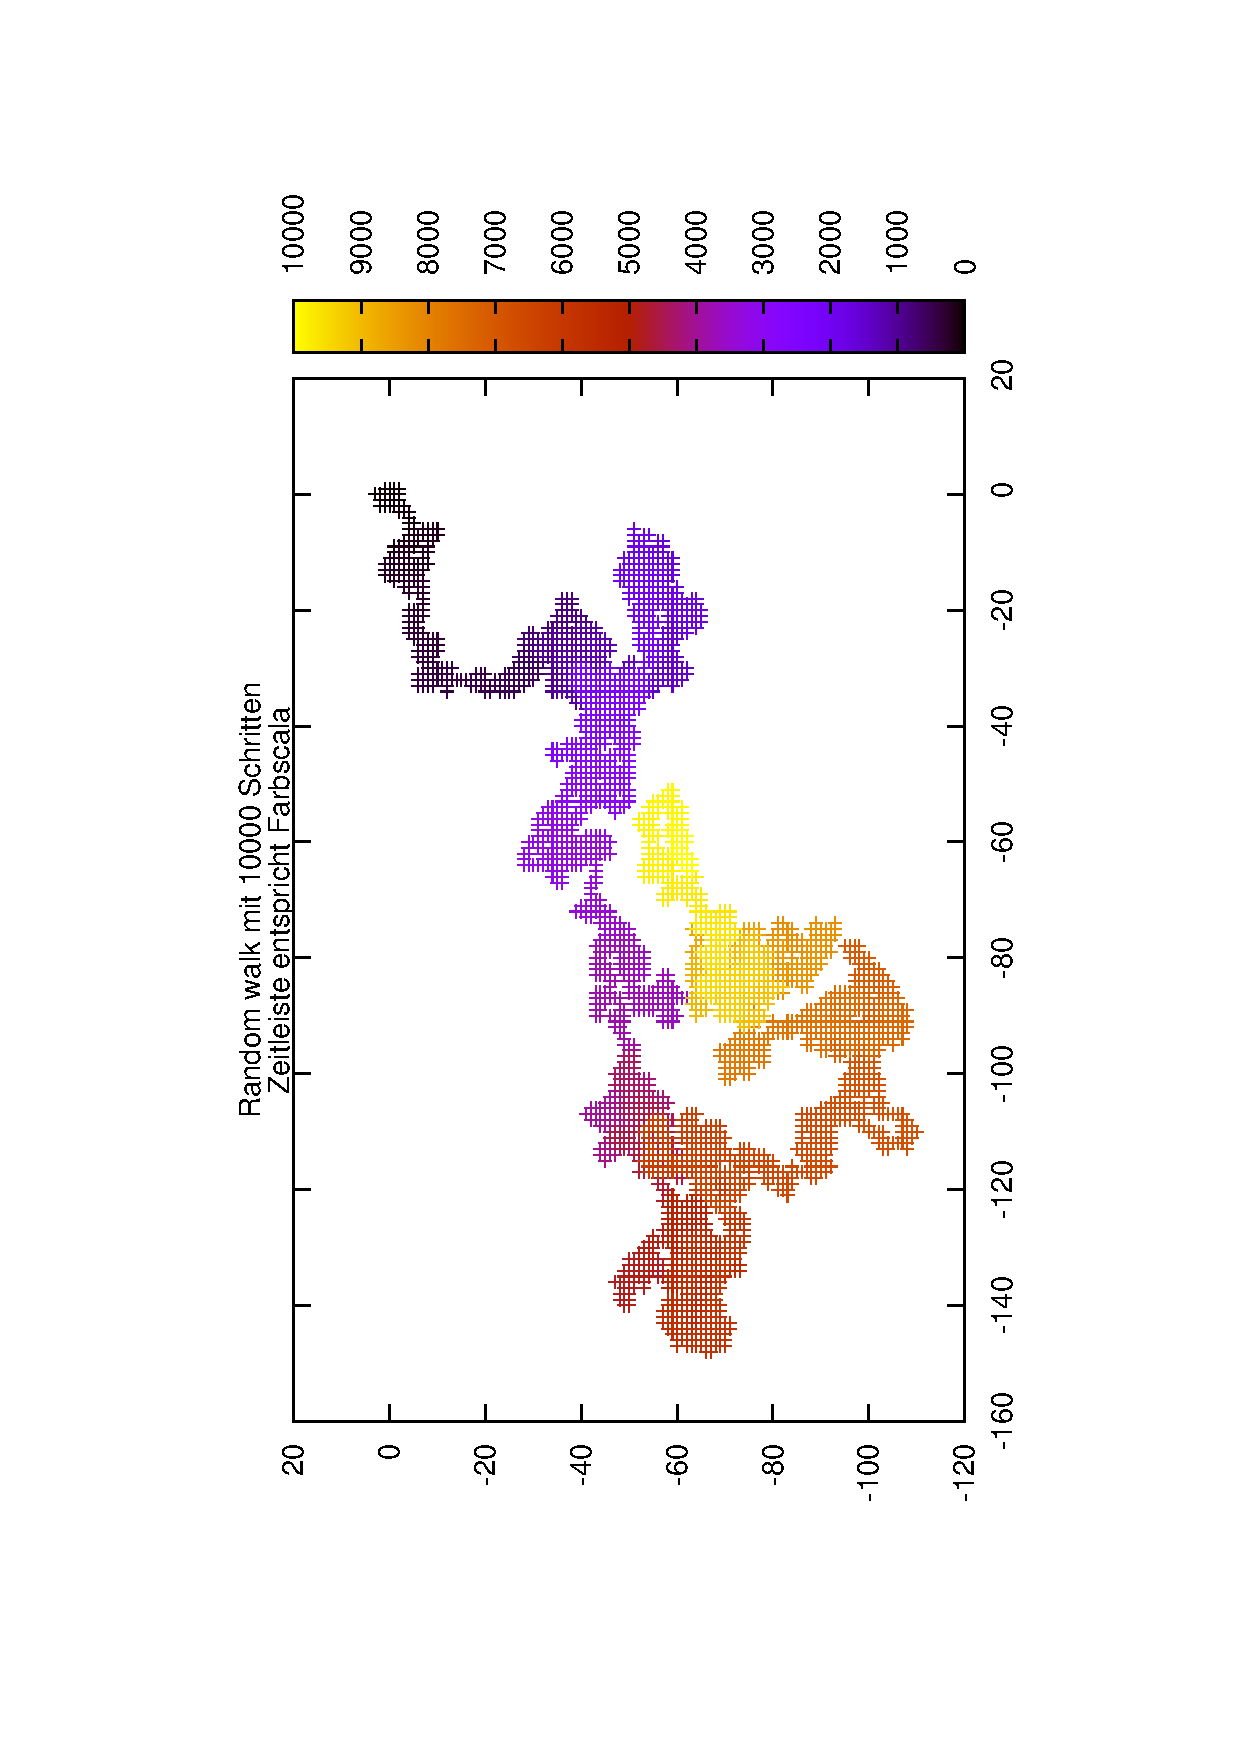
\includegraphics[angle=-90,width=0.45\textwidth]{rw-10000-2}}
  \subfigure{\includegraphics[angle=-90,width=0.45\textwidth]{rw-10000-1}}
  \subfigure{\includegraphics[angle=-90,width=0.45\textwidth]{rw-100000-2}}
  \subfigure{\includegraphics[angle=-90,width=0.45\textwidth]{rw-100000-0}}
  \caption{Random Walks; von oben nach unten $10^1, ..., 10^5$ Schritte}
  \label{fig:random-walks}
\end{figure}

\begin{figure}
  \centering
    \subfigure{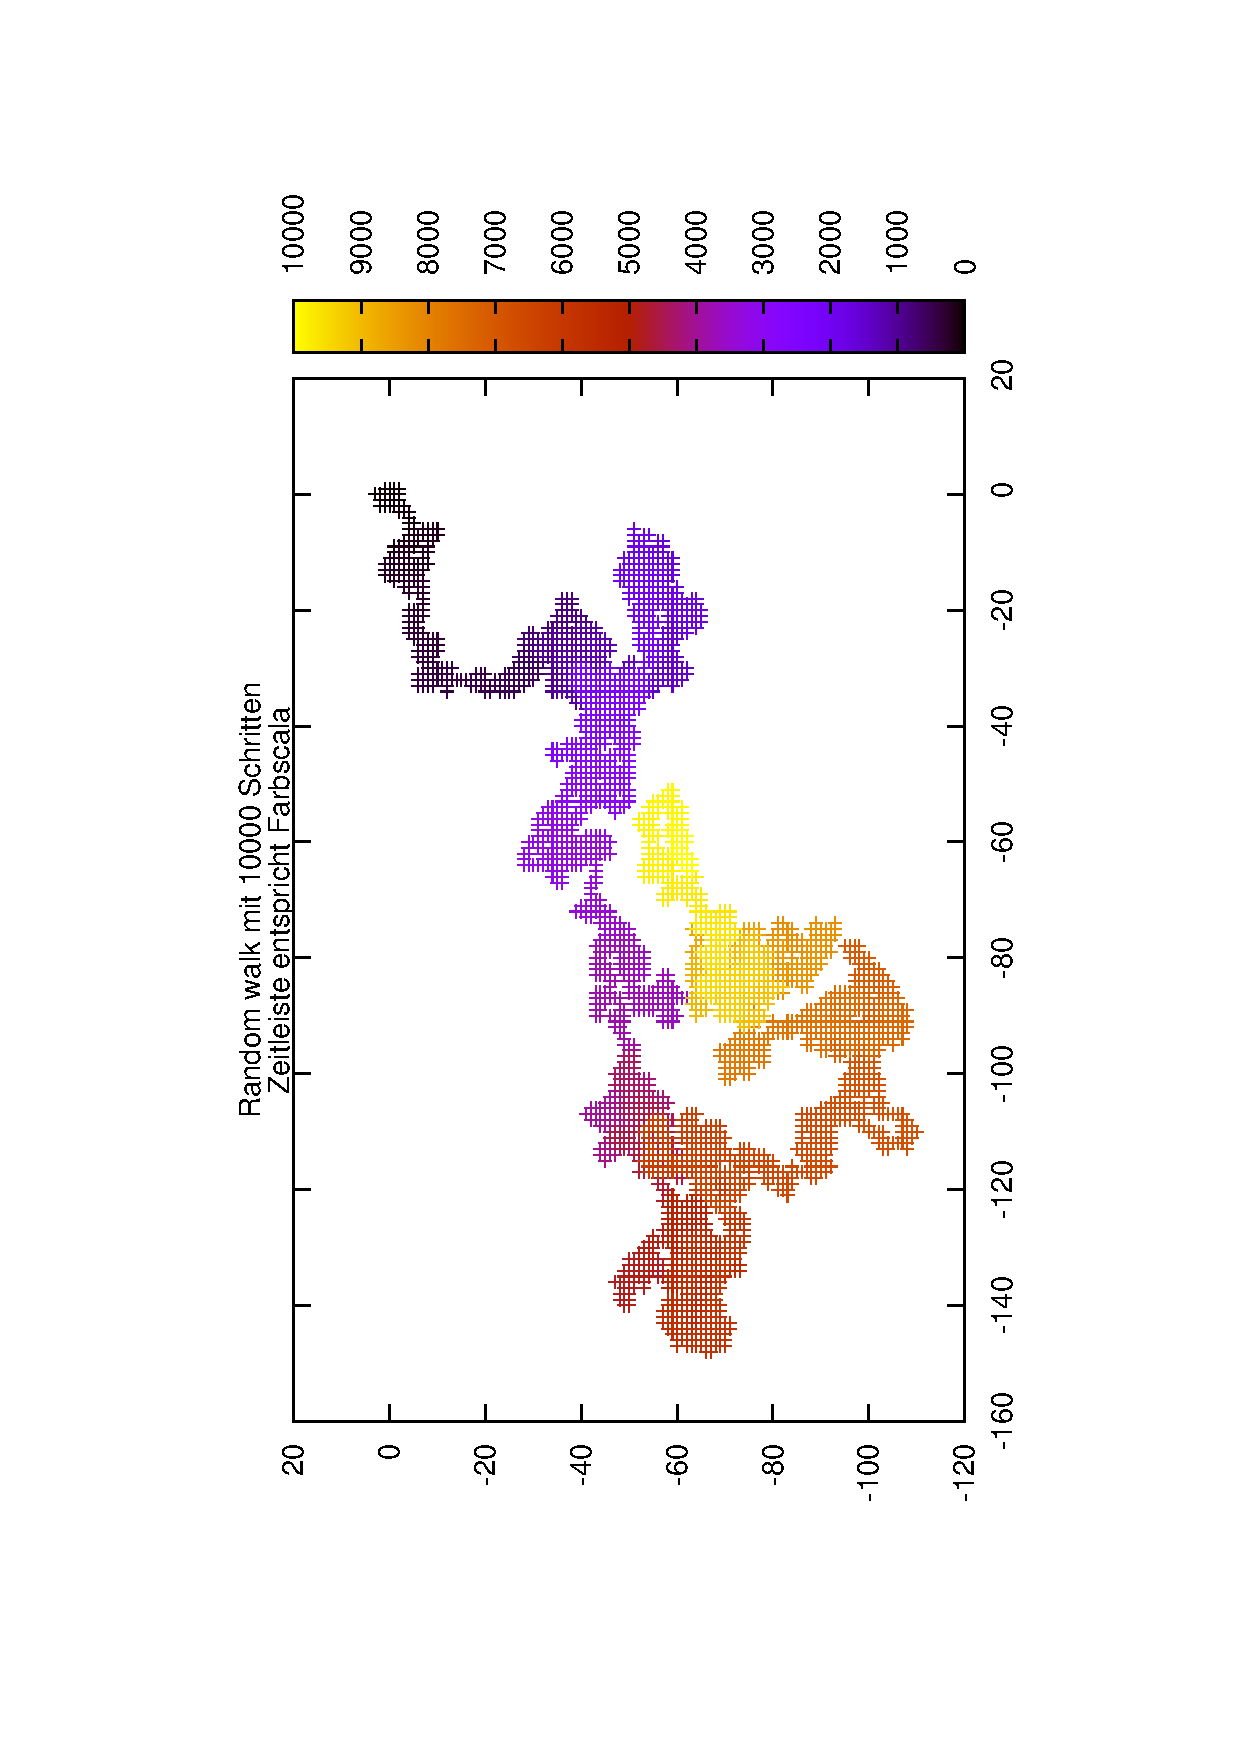
\includegraphics[angle=-90,width=\textwidth]{rw-10000-2}}
    \subfigure{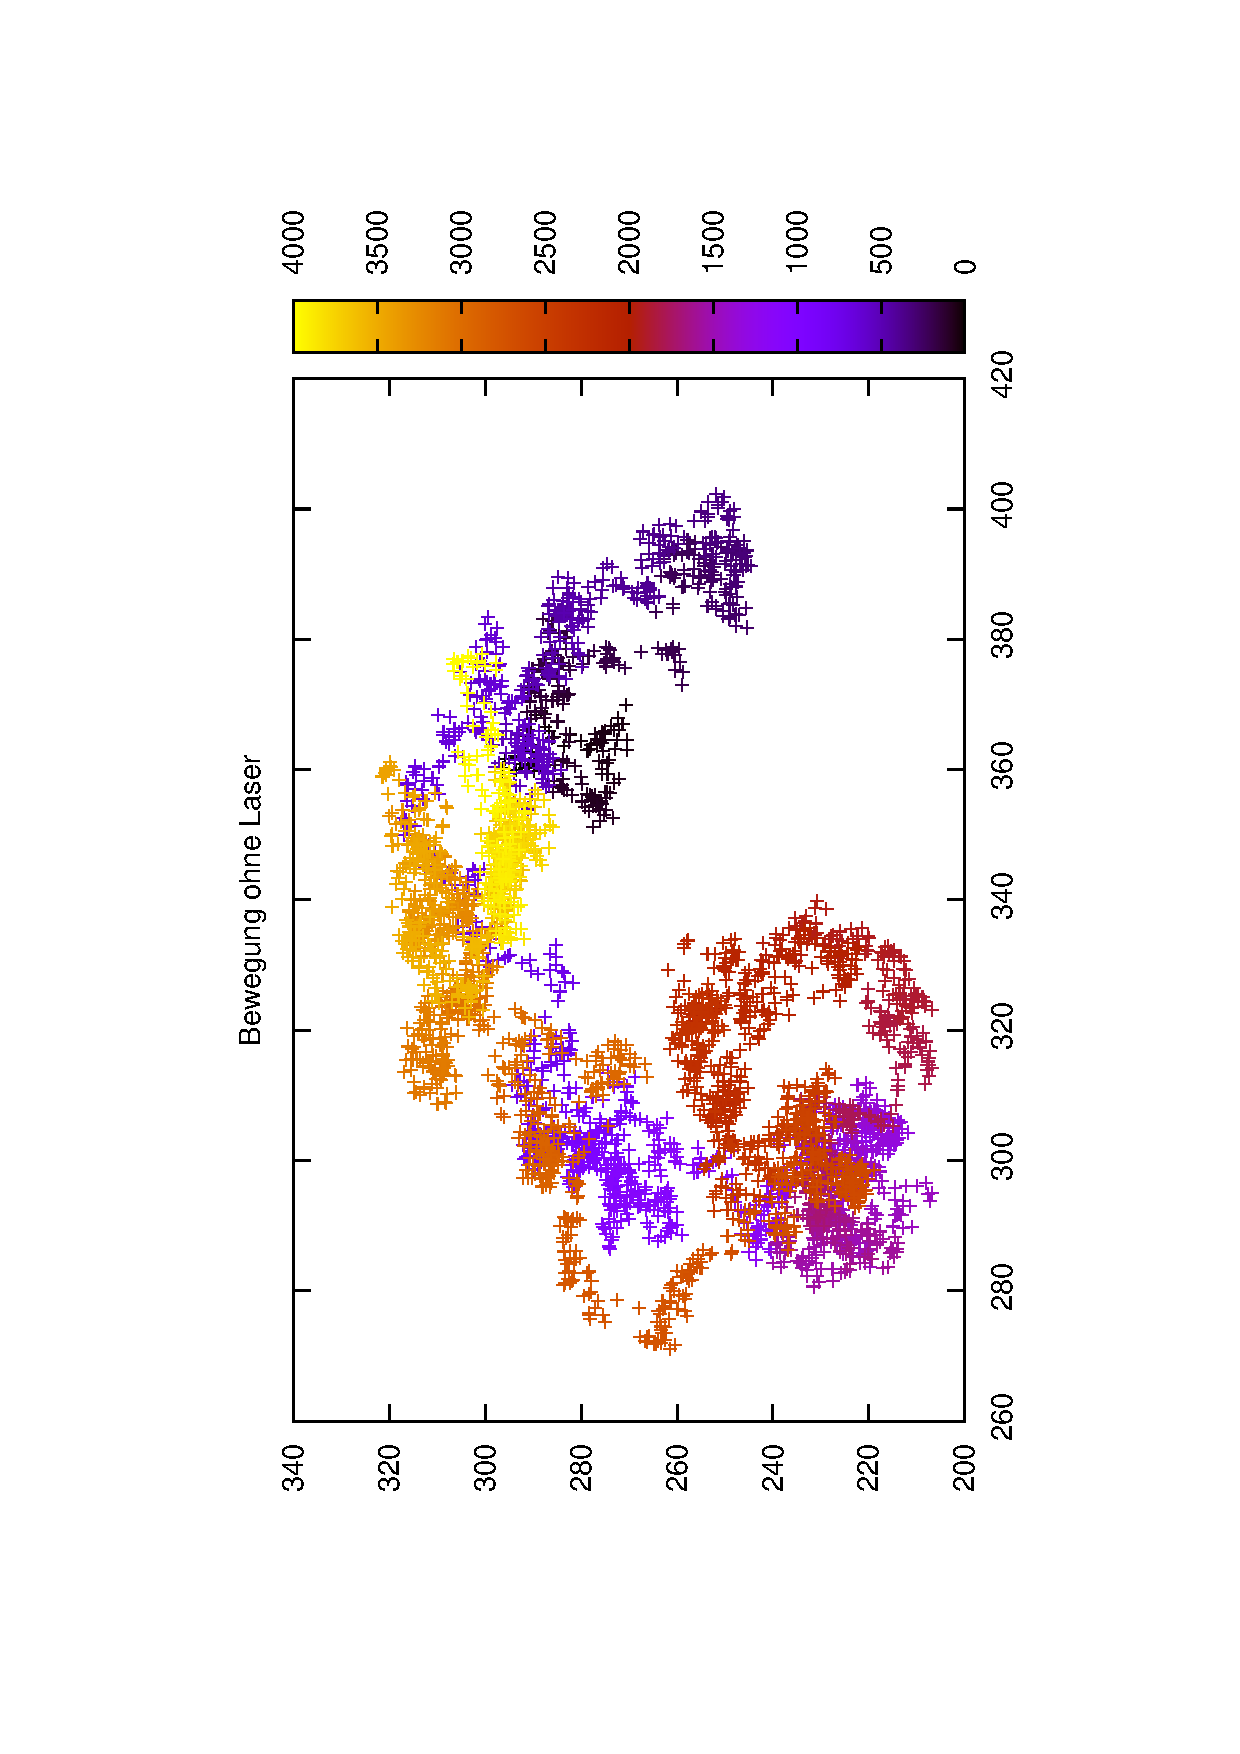
\includegraphics[angle=-90,width=\textwidth]{rw-real}}
  \caption{Vergleich der Simulierten und einer realen Bewegung mit Ranom Walk}
  \label{fig:vgl-real-rw}
\end{figure}

\abs
Mit \texttt{randomw02.cpp} sieht man, dass die Teilchen sich beim
Random Walk im Mittel nicht vom Ausgangsort entfernen:
\begin{equation}
  \label{eq:1}
  \langle \vec R  \rangle = ( 0.151 , 1.759 ) \;,
\end{equation}
wobei die verschiedenen Endpunkte sehr breit verteilt sind:
\begin{equation}
  \label{eq:2}
  \langle \vec R^2  \rangle = ( 499.113 , 495.643 ) \;.
\end{equation}

\abs
Um das Histogramm zu erzeugen, kann man \texttt{histo03.cpp}
verwenden; hierzu muss man die Zahl der Moves eingeben. Mit bspw.
\begin{lstlisting}[language=bash]
g++ -o histo03 histo03.cpp
g++ -o randomw02 randomw02.cpp
./randomw02 | ./histo03 1000
\end{lstlisting}
kann man so ein sch"ones Histogramm erzeugen; mit Gnuplot geplottet
sind die Daten in Abb. \ref{fig:distrrandomw1000} zu finden.

Verwendet man $500\,000$ Walks, so bekommt man eine sch"onere
Gau"s-Verteilung; dies ist in Abb. \ref{fig:distrrandomw500000}
angefittet.



\begin{figure}
  \centering
  \includegraphics[width=\textwidth]{randoms-1000.histo.eps}
  \caption{Verteilung der X-Koordinate nach 1000 Random Walks}
  \label{fig:distrrandomw1000}
\end{figure}

\begin{figure}
  \centering
  \includegraphics[width=\textwidth]{randoms-500000.histo.eps}
  \caption{Verteilung der X-Koordinate nach 500000 Random Walks;
    Gau"sglocke angefittet}
  \label{fig:distrrandomw500000}
\end{figure}


\end{document}














%%% Local Variables: 
%%% mode: latex
%%% TeX-master: t
%%% End: 
